\documentclass[11pt, oneside]{article} 
\usepackage{geometry}
\geometry{letterpaper} 
\usepackage{graphicx}
	
\usepackage{amssymb}
\usepackage{amsmath}
\usepackage{parskip}
\usepackage{color}
\usepackage{hyperref}

\graphicspath{{/Users/telliott_admin/Dropbox/Tex/png/}}
% \begin{center} 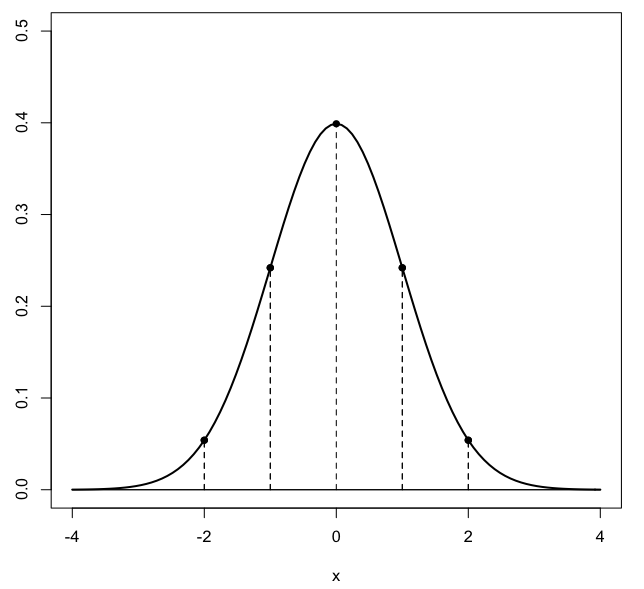
\includegraphics [scale=0.4] {gauss3.png} \end{center}

%break
\title{Poisson distribution}
\date{}

\begin{document}
\maketitle
\Large

The Poisson distribution is a special case of the famous binomial distribution for Bernoulli trials.  It is an approximation for situations in which the probability of success $p$ on each trial is small, and the number of trials $n$ is large, so that the mean $\lambda = np$ of successes is not too much greater than $1$ for the sequence of trials taken as a whole.

Recall that the binomial distribution for the number of successes $k$ on $n$ trials, with probability $p$ of success on each trial is:

\[ P(k) = {n\choose k} \  p^k \  (1-p)^{n-k} \]

where

\[ {n\choose k} =  \frac{n!}{k!  \ (n-k)!}  \]

Briefly, the derivation of this formula is that in independent trials with probability of success $p$ and of failure $q$, for a particular series of successes and failures, say:

\[ \textbf{S\ S\ F\ S\ S\ F\ F\ F\ F\ S\ S\ F\ F} \]

the probability is

\[ P = p \ p \ q \ p \ p \ q \ q \ q \ q \ p \ p \ q \ q = p^6 q^7 \]

and more generally, for $k$ successes in $n$ trials

\[ P = p^k q^{n-k} \]

Since $q = 1-p$

\[ = p^k (1-p)^{n-k} \]

The factor of
\[ \frac{n!}{ k! \ (n-k)! } \] 

which is $\ge 1$, recognizes the occurrence of the combinations, that is, all the permutations of 

\[ \textbf{SSFSSFFFFSSFF} \]

such as 

\[ \textbf{SSSSSSFFFFFFF} \]

 that have the \emph{same} number of total successes.  Each of these contributes to the probability of $k$ successes in $n$ trials---see
 
\url{http://en.wikipedia.org/wiki/De_Finetti's_theorem}

\subsection*{Simplifying ${n\choose k}$}

The first step involves the "choose" or combinations term. We are interested in applications where $n$ is large and $p$ is small, and the mean number of successes is roughly near 1.  For $k=2$

\[ {n\choose 2} =  \frac{n!}{k!  \ (n-k)!}  \]
\[ = \frac{ n (n-1)}{k!} \ \frac{(n-2) (n-3) \cdots}{(n-2) (n-3) \cdots} \]
\[ = \frac{ n (n-1) }{ k! } \]
Since $n$ is large
\[  {n\choose 2} = \frac{ n (n-1) }{ k! } \approx \frac{n^2}{2!} \]

and more generally

\[ {n\choose k} \approx \frac{n^k}{k!}  \]

\subsection*{part 2}

The other term we will modify is

\[ (1-p)^{n-k} \]
\[ = \frac{(1-p)^n}{(1-p)^{k}} \]

The probability $p$ is quite small, but because $n$ is very large, we cannot just set $1-p$ equal to $1$ for the numerator, $(1-p)^n$.

In contrast, if $k$ is a modest size (say, $k < 10$),we \emph{can} reasonably set $1-p = 1$ for the second term, and thus the denominator is equal to $1$. The first term contributes much more than the second to the value for this expression.

Finally, we will show that $(1-p)^n \approx e^{-np}$.

Recall that

\[ e^x = 1 + x + \frac{x^2}{2!} + \cdots \approx 1 + x \]
(for small $x$)

Since $|p|$ is small, we have

\[ e^{-p} \approx 1 - p \]

so

\[ (1-p)^n \approx (e^{-p})^n = e^{-np} \]

Alternatively, we note that the binomial expansion (for $x$ near zero) is 
\[ (1 + x)^n \approx 1 + x \]
by a Taylor series.  Since both $(1-p)^n$ and $e^{-p}$ are approximately equal to $1-p$ they are approximately equal to each other.

\subsection*{Finishing up}

Substituting, we get

\[ P(k) = {n\choose k} \  p^k \  (1-p)^{n-k} \]
\[ \approx \frac{n^k}{k!} \ p^k \ e^{-np} \]

We introduce a symbol for the mean, $\lambda = np$

\[ P(k) \approx \frac{n^k}{k!} \ p^k \ e^{-\lambda} \]
\[ \approx  \frac{\lambda^k}{k!} \ e^{-\lambda} \]

This is the Poisson distribution for the number of successes $k$ in $n$ Bernoulli trials where the mean number of successes $\lambda = np$ over the whole series of trials is small.

\subsection*{The Poisson is normalized}

The Poisson distribution is normalized, i.e. it sums to $1$, and so is a proper probability distribution.

\[ \sum\limits_{k=0}^{\infty} \frac{\lambda^k}{k!} \ e^{-\lambda} = e^{-\lambda} \ \sum\limits_{k=0}^{\infty} \frac{\lambda^k}{k!} = 1 \]

since

\[ \sum\limits_{k=0}^{\infty} \frac{{\lambda}^k}{k!} = \frac{{\lambda}^0}{0!} + \frac{{\lambda}^1}{1!} + \frac{{\lambda}^2}{2!} + \cdots  = e^{\lambda} \]


\subsection*{Note}

I've always used a different set of symbols (from David Freifelder's \emph{Molecular Biology}), although the ones shown above are standard in statistics.  In his notation the mean is $m$ and the number of successes is $i$ so the equation is

\[ P(i) = \frac{e^{-m} \ m^i }{ i! } \]

which I remember as "Emmy!" or more explicitly, "emmii!".

One important propety of the Poisson distribution is that it always simplifies dramatically for $P(0)$, and also for $P(1)$ in the case where the mean is equal to $1$.

\[ P(i) = \frac{e^{-m} \ m^i }{ i! } \]
\[ P(0) = \frac{e^{-m} \ m^0 }{ 0! } \]
\[ P(0) = e^{-m} \]

When the mean is one, $m = 1$

\[ P(0) = \frac{1}{e} \]
\[ \approx 0.368 \]

and 

\[ P(1) = \frac{e^{-1} \ 1^1 }{ 1! } = \frac{1}{e} \]

For example, if we had a box that is divided into one hundred compartments, and if it were possible to throw one hundred marbles into it at random (equal probability for each bin), then at the end of the experiment slightly more than $1/3$ of the compartments will still be empty, an equal number will contain one marble, and about 25 percent will contain more than $1$.  (Grinstead and Snell use the example of V1 rockets aimed at the city of London).

The same holds for a bacterial culture infected with virus at a ratio of one virus per bacterial cell.  At an $ moi = 1$ ("m.o.i." is short for "multiplicity of infection"), more than one-third of the cells will be uninfected.

Here is a plot of the Poisson distribution for selected values of $\lambda$ ($m = 1,2,5,10$).

\begin{center} 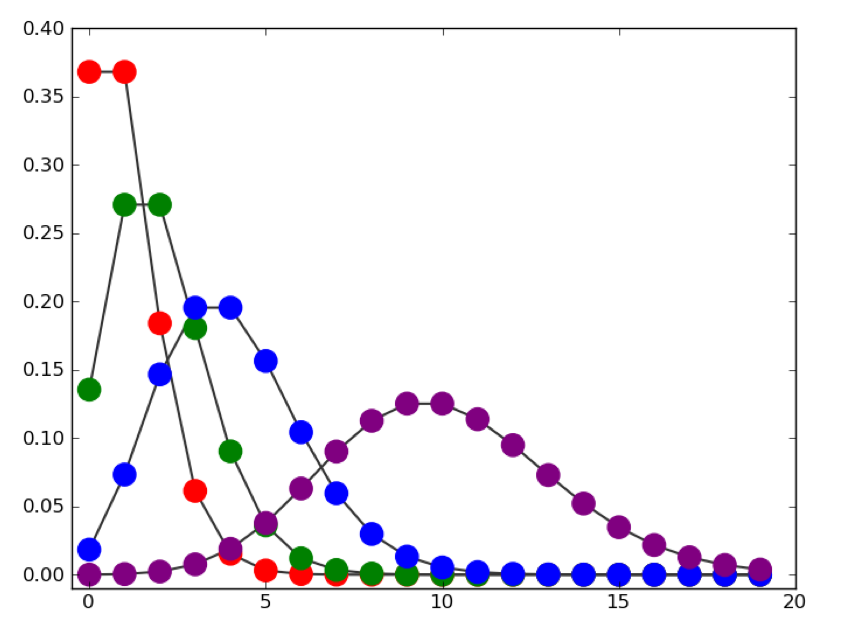
\includegraphics [scale=0.4] {poisson.png} \end{center}

Note the very small values for $P > 10$ when $m < 5$ (red, green, and blue).  That's the inverse factorial talking.

\subsection*{Genetics}

One application is to bacterial genetics.  Consider the Luria-Delbruck experiment, in which mutant bacteria resistant to the action of the bacterial virus T1 were selected.  A modern (Darwinian) view appreciates that the mutations which confer virus-resistance pre-exist in the population, having occurred randomly during growth.  

An alternative, the Lamarckian view, suggests that the mutations arise \emph{in response} to each bacterium's encounter with the virus.

So if we have an agar plate whose surface contains $10^8$ bacterial cells and an excess of virus particles, we can model the Lamarckian view as a process in which each individual cell has an extremely small probability of surviving the phage assault to which it is subjected, but the large number of cells constitutes a large number of trials.  We adjust the mean number of successes (phage-resistant colonies per plate) to be near $1$.  Then, the Poisson approximation should apply.

In particular, if $f$ is the fraction of plates which have no resistant colonies, then in

\[ P(i=0) = \frac{e^{-m} \ m^i }{ i! } \]

both $m^i$ and $i!$ equal $1$ and so

\[ P(i=0) = f = e^{-m} \]
\[ m = - \ln f \]

For example, if $f=0.5$, then $m=0.69$.  Now we can calculate $P(i=1)$, $P(i=2)$, and the whole distribution.  Here is the probability distribution for $m=1$ and $i=0 \cdots 5$:

\[
\begin{matrix}
0 & 0.368 \\
1 & 0.368 \\
2 & 0.184 \\
3 & 0.061 \\
4 & 0.015 \\
5 & 0.003 \\
\end{matrix}
\]

and here is the cumulative distribution:

\[
\begin{matrix}
0 & 0.368 \\
1 & 0.736 \\
2 & 0.92 \\
3 & 0.981 \\
4 & 0.996 \\
5 & 0.999 \\
\end{matrix}
\]

The probability of observing 6 or more colonies is less than $1/1000$.

Crucially, this is \emph{not} what one observes.  Instead, trials (plates) containing dozens or even hundreds of colonies are obtained at a frequency of about 1 plate in 10.  These are Luria's "jackpots."

In summary, the results are inconsistent with the Lamarckian view, but are easily explained by a model in which mutations occur randomly with respect to each cell division.  If a mutation happens to occur early in the growth of a culture, that mutant cell will have a large number of descendants, each of which can form a phage-resistant colony.

\end{document}  